\documentclass[sigconf, nonacm]{acmart}
\settopmatter{printfolios=true}
\settopmatter{printacmref=false}
%% PACKAGES
\usepackage{graphicx}
\usepackage{hyperref}
\usepackage{cleveref}
\usepackage{subcaption}
\usepackage{natbib}
\usepackage{mathtools}
\usepackage{xcolor}

%% COLORS
\definecolor{darkgreen}{rgb}{0,0.8,0}

%% TITLES
\title{Review of Estimating 3D Motion and Forces of Person-Object Interactions from Monocular Video}

%% AUTHORS
\author{Balthazar Neveu}
\affiliation{%
  \institution{ENS Paris-Saclay}
  \city{Saclay}
  \country{France}
}
\email{balthazar.neveu@ens-paris-saclay.fr}

\author{Matthieu Dinot}
\affiliation{%
  \institution{Ecole Polytechnique}
  \city{Palaiseau}
  \country{France}
}
\email{matthieu.dinot@polytechnique.edu}

%% MAIN DOCUMENT
\begin{document}

  %% KEYWORDS
  \keywords{Perception and Estimation, Optimal Control, Inverse Problems}

  %% Teaser figure
  \begin{teaserfigure}
    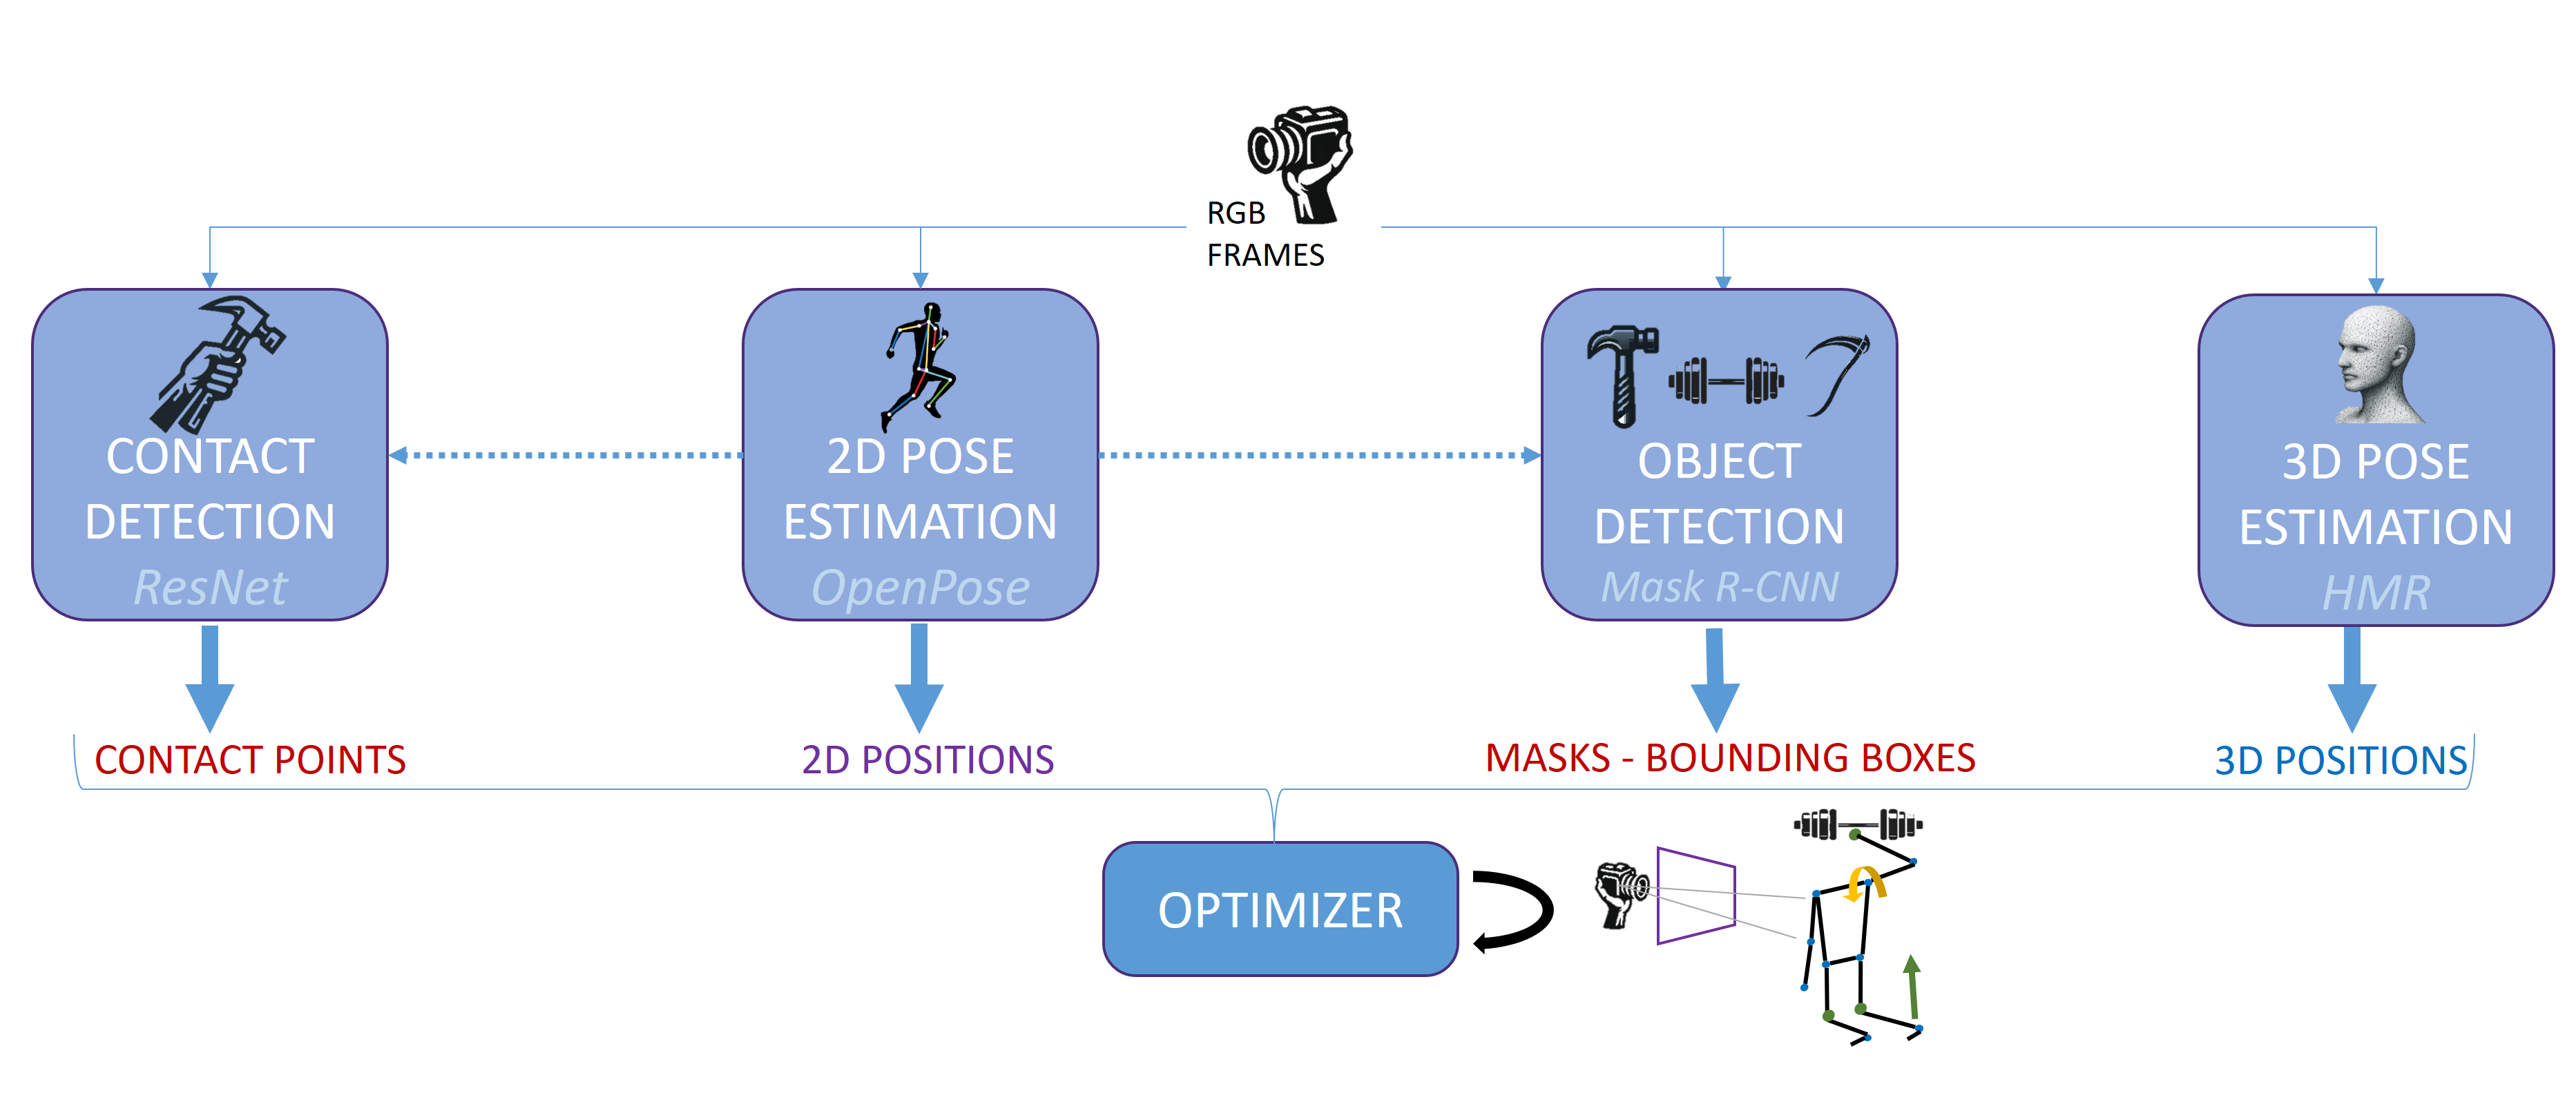
\includegraphics[width=0.6\textwidth]{figures/authors_original_pipeline.png}
    \centering
    \caption{Full original pipeline. 
    A multiple stage vision pipeline extracts poses and contact data of the human and the object.
    Full body dynamics (joint angles, torques and external forces) are then reconstructed during the optimization stage.
    }
    \label{fig:original_pipeline}
  \end{teaserfigure}

  %% TITLE
  \maketitle




  %% CONTENT
  \section{Introduction}
\label{sec:intro}

Humans can easily learn how to perform a given movement or manipulate an object by observing others and attempting to replicate their actions. 
In robotics, this behavioral cloning ability would be usefull to train humanoid robots to perform such tasks. 
However, unlike humans, computers still struggle to understand complex human-object interactions from visual data alone. 
Traditional methods like motion capture offer a solution, but they come with high costs and do not leverage the abundant instructional video 
resources available online.

To address this challenge, \citet{li2019estimating} proposed a novel approach for estimating 3D motion and forces of human-object interactions 
from single RGB videos. 

In this work, we critically reviewed and reimplemented certain aspects of their method. Our initial goal was to assess 
the reproducibility and robustness of the original findings, as well as to explore potential enhancements. We focused on understanding the 
underlying methodology, adapting it to a simplified pipeline. Our code is available on~\href{https://github.com/balthazarneveu/monocular_pose_and_forces_estimation}{GitHub}.



  \section{Methodology of the Original Paper}
\label{sec:methodo_paper}

The study by \citet{li2019estimating} aimed to reconstruct the 3D motion of a person interacting with an object, including the position 
and applied forces, from a single RGB video. Their methodology unfolds in two principal steps. The first step involves the application of 
computer vision techniques to accurately determine the human and object poses, as well as the points of contact between them and with the 
surrounding environment. The second step solves an optimization problem, rooted in control theory principles, to fully recover 
the dynamic motion.  


\subsection{Retrieve Human and Object 3D Pose and Contact from RGB Video}
\label{subsec:retrieve_original}

\noindent\textbf{Human 2D Pose Estimation.}\label{2dpose} For the task of human pose estimation, the authors utilized a pretrained version of 
OpenPose~\cite{cao2017realtime}. This tool enabled them to identify and track human joint positions in two dimensions from the RGB video.

\noindent\textbf{Contact Recognition.} The recognition of contact points, being whether specific joints (like feet, hands, and neck) were in 
contact with the ground or the object, was achieved by first cropping areas in the video frame around the joints identified by OpenPose. 
These cropped images were then processed through the corresponding joint's ResNet \cite{he2016deep}, which had been trained on a custom dataset 
to discern contact.

\noindent\textbf{Object 2D Endpoint Detection.} For estimating the 2D positions of object endpoints, the authors utilized instance segmentation 
capabilities of Mask R-CNN \cite{he2017mask}. This method was applied to different classes of objects (such as barbells, hammers, scythes, 
and spades) identified in their video dataset. Mask R-CNN, trained separately for each object class, enabled the extraction of segmentation masks
and bounding boxes from the video frames. These were then used to estimate the 2D locations of the object's endpoints.

\noindent\textbf{Human 3D Pose Estimation.} The authors also utilized HMR~\cite{kanazawa2018end} for 3D human pose estimation, although this 
is not clearly stated in their method overview.


\subsection{Reconstruct Person-Object Dynamic Motion}
\label{subsec:reconstruct_original}

The optimization framework presented by \citet{li2019estimating} is designed to estimate the 3D trajectories of both the human and the object, 
as well as the exerted contact forces, by solving the following trajectory optimization problem: 

\begin{equation*}
    \begin{aligned}
        & \underset{x,u,c}{\text{minimize}}
        & & \int_{0}^{T} l^h(x, u, c) + l^o(x, u, c)dt, \\
        & \text{subject to}
        & & \kappa(x, c) = 0 \quad (\text{contact motion model}), \\
        &&& \dot{x} = f (x, c, u) \quad (\text{full-body dynamics}), \\
        &&& u \in \mathcal{U} \quad (\text{force model}).
    \end{aligned}
\end{equation*}

\noindent\textbf{Variables.} The state variables \(x \coloneqq (q^h, q^o, \dot{q}^h, \dot{q}^o)\) encompass the configuration and velocities of 
the human and object, while the control variables \(u \coloneqq (\tau_m^h, f_k, k=1, \dots, K)\) include the muscle torques and contact forces 
at the \(K\) contact points. The contact state \(c\) represents the presence and locations of contacts throughout the video sequence. 

It should be noted, although not explicitly stated in the paper, that in their implementation, the velocities (\(\dot{q}^h\) and \(\dot{q}^o\))
are not directly used as variables. Instead, velocities are approximated using the backward finite difference scheme 
\(\dot{q}_t = (q_t - q_{t - 1}) / \Delta t\).

\noindent\textbf{Loss Functions.} The loss functions \(l^h\) and \(l^o\) for the human and object respectively consist of the following components:

\begin{itemize}
    \item 
        \(l_{2D}\): A term ensuring 2D consistency by minimizing the error between the observed 2D joint positions given by OpenPose and 
        their re-projections from the 3D estimates, using the camera projection matrix \(P_{\text{cam}}\). Outlier influence is mitigated 
        by employing the Huber loss function \(\rho\).
    \item 
        \(l_{3D}\): This loss ensuring that the estimated 3D positions adhere closely to the HMR references.
    \item 
        \(l_{\text{pose}}^h\): A likelihood term for the human pose, encouraging plausible human poses through a Gaussian Mixture Model 
        trained on motion capture data.
    \item
        \(l_{\text{torque}}^h\): A regularization term penalizing high muscle torque values to favor energy-efficient movements.
    \item 
        Motion smoothness: Terms penalizing rapid movements or accelerations to align with the typically smooth human motion observed over 
        the video frame rate.
    \item
        Force-related terms: These encompass additional forces and contact forces that were not the focus of further investigation in our 
        study.
\end{itemize}

The loss function for the object, \(l^o\), is constructed similarly, omitting the 3D consistency and pose likelihood terms due to the nature 
of object motion and the absence of a pose prior.
  \section{Reimplementation Strategy}
\label{sec:remplementation}

The code accompanying the orignial paper is rather difficult to use due to its inherent complexity and lack of documentation. 
To effectively explore the core contributions of the paper, we decided to reimplement parts of it with a more focused scope.

In our approach, we focused on reconstructing arm motion from video data,
a simplification that allowed us to tackle the fundamental 
aspects of the methodology without the computational burden of full-body modeling.

Our code is available and documented on~\href{https://github.com/balthazarneveu/monocular_pose_and_forces_estimation}{GitHub}.

\subsection{Overview}
\label{subsec:overview}
Our simplification regarding the original paper are listed below:
\begin{itemize}
    \item Only the arm motion (shoulder, elbow and wrist) is considered and not the full body.
    \subitem - We end up with the arm state $q$ being a quaternion describing 
    the upper arm state and a single elbow angle for the forearm state.
    \subitem - Shoulder is fixed to the world frame.
    \item Do not deal with objects and external contact forces.
    \item Act under controlled conditions.
    \subitem - A correct lighting and a static background to simplify the vision task.
    \subitem - We make sure that the camera is on a tripod and geometrically calibrated.
\end{itemize}

Regarding implementation, we started from scratch. Instead of trying to re-implement
the whole inverse dynamics optimization framework at once, we progressively built a solution.
Since the arm has only 4 degrees of freedom, leading to 3x 3D joints, 
fitting the full camera parameters (extrinsics and intrinsics) at the same time
as fitting the whole arm dynamics is not possible (under determined system).
\begin{itemize}
    \item (\ref{subsec:vision_pipeline}) - Vision pipeline 
    extracts 3x 2D and 3x 3D arm estimated joints positions.
    \item (\ref{subsec:inverse_kinematics}) - We use inverse kinematics  
    on the 3D points to get coarse robot arm state.
    \item (\ref{subsec:cam_estim}) - We fit the camera/shoulder translation 
    by minimizing the 2D reprojection error of the 3D points.
\end{itemize}



% WARNING: !!!!!!!!!!!! 
Due to lack of time, we were not able to implement the inverse kinematics which minimizes jointly
the camera pose and the arm state $q$.

Finally, using the above $q$ state estimation as an initialization,
we implemented a proof of concept for the inverse dynamics optimizer (\ref{subsec:inverse_dynamics}) focusing on:
\begin{itemize}
    \item minimizing $l_{\text{3D}}$ the 3D reprojection error of the arm joints.
    \item under relaxed dynamic constraint.
    \item under smooth motion constraints (velocities and accelerations)
\end{itemize}
% WARNING: !!!!!!!!!!!! 


\subsection{Vision Pipeline}
\label{subsec:vision_pipeline}

For 2D and 3D human pose estimation, we utilized the MediaPipe framework~\cite{lugaresi2019mediapipe}, which offers a more modern alternative 
to OpenPose. MediaPipe simplifies the vision pipeline by also replacing HMR in our usecase. An illustration of MediaPipe's inference results 
can be seen in~\cref{fig:mediapipe}. We then only used the arm joint 2D and 3D positions. 

\begin{figure}
    \centering
    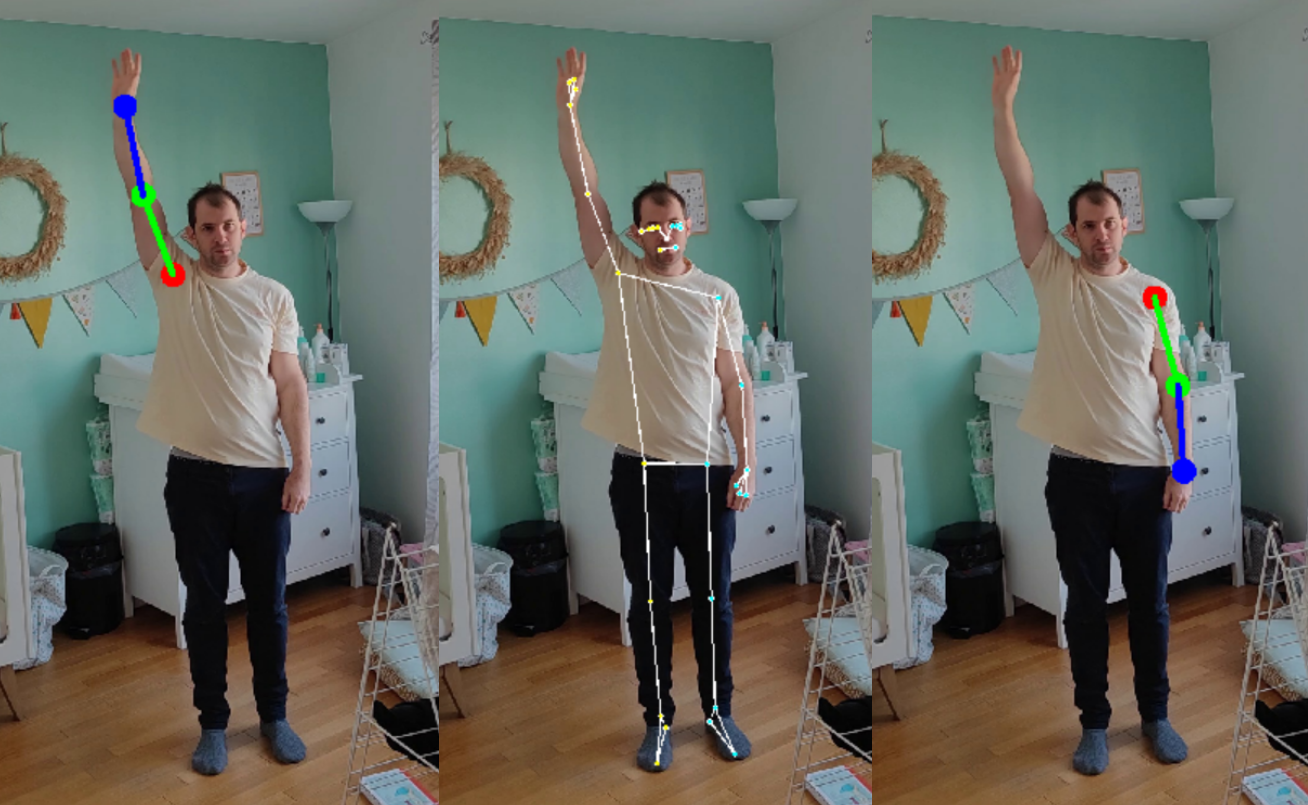
\includegraphics[width=8cm]{figures/pose_detection_mediapipe_collage.png}
    \caption{
    \color{red}Shoulder, \color{darkgreen}elbow, \color{blue}wrist \color{black} joints indicated with dots
    are linked by the \color{darkgreen}upper arm \color{black} and \color{blue}forearm \color{black}. 2D and 3D data is extracted from
    the full body pose estimated with MediaPipe.
    }
    \label{fig:mediapipe}
\end{figure}

Although we experimented with the contact recognizer component, we did not use it into our pipeline since we do not model contact.

\subsection{Arm Model}
\label{subsec:arm_model}
We modelled the arm in Pinocchio~\cite{carpentier2019pinocchio}. The shoulder is represented by a spherical joint, allowing for three degrees 
of freedom. This is expressed as a quaternion in the state vector \(q\). The elbow is represented by a revolute joint, which permits rotation 
within a plane, resulting in a single degree of freedom. The state \(q\) therefore consists of five elements: the first four correspond to the 
shoulder quaternion, and the fifth represents the elbow angle, which is constrained within the range \([0, \pi]\) radians. The dimensions of 
the arm are fixed with the forearm and upper arm lengths fixed at 27 cm and 23 cm, respectively. See~\cref{fig:arm_model}

\begin{figure}
    \centering
    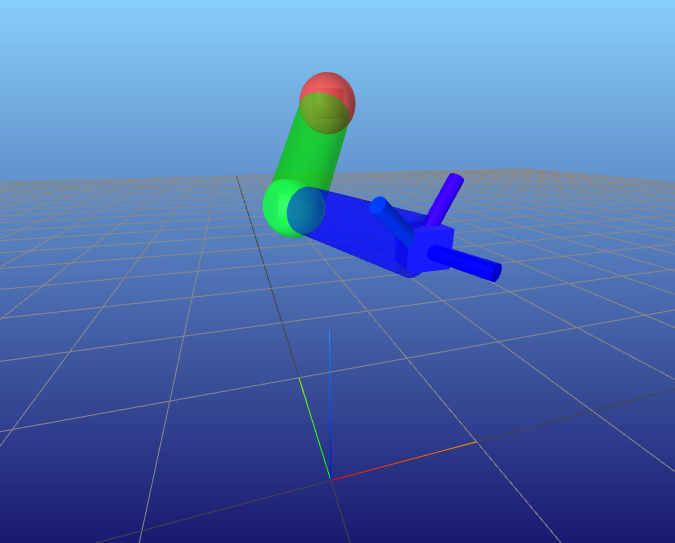
\includegraphics[width=0.3\textwidth]{figures/live_arm.png}
    \caption{Arm Model vizualisation}
    \label{fig:arm_model}
\end{figure}

\subsection{Inverse Kinematics}
\label{subsec:inverse_kinematics}
To get proper initializations to feed to the inverse dynamics optimizer, we relied on the 3D positions of the arm joints estimated by MediaPipe~\cite{lugaresi2019mediapipe}.
From a sequence of 3D positions of the arm joints, we used the inverse kinematics approach to estimate the joint angles.
Inverse kinematics is higly relying on the Pinocchio library ~\cite{carpentier2019pinocchio} to compute 
the Jacobian and perform forward kinematics (compute the 3D positions  $M(t)_{j}$ of the joints from the joint angles $q(t)$).
% @TODO: Add equations for IK with the 2 tasks (elbow and wrist 3D positions)

Devil is in the details, and we had to be careful about the following points while implementing:
\begin{itemize}
    \item We provide 2 tasks to the inverse kinematics solver: one for the elbow 3D position and one for the wrist 3D position. 
    Order matters, elbow comes first.
    \item The mediapipe 3D estimations are not perfect but the most nottable issue is that 
    the upper arm and the forearm lengths are not constant across time. To overcome this limitation,
    3D positions are re-scaled to match the expected nominal model arm length. 
    This arm length normalization ensures that a solution exists but on the other hand, it may introduce reprojection errors.
\end{itemize}
Although nothing grants temporal smoothness of the estimated joint angles, we recursively feed the previous solution as an initial guess to the current timestep.
This simple trick gives good results in practice (assessed qualitatively on the match between the moving arm and the video).


\subsection{Camera position}
\label{subsec:cam_estim}

\noindent\textbf{Problem formulation.} Since the upper arm can rotate in all directions and since we're not using any priors to constrain 
the arm motion (at the shoulder level), moving the camera around the arm is equivalent to spinning the arm around itself. 
Our simplification unfortunately leads to a degenerate problem where the camera rotation may end up being redundant with the arm rotation.
To avoid this issue, we decided to fix the camera orientation. 
We estimate the camera 3D position $P_{\text{cam}}(t)$ 
by jointly minimizing the 2D reprojection error of joints.
$$\underset{P_{\text{cam}}(t)}{min}\sum_{j\in{\text{shoulder, elbow, wrist}}} \|K\cdot\left[Q_{\text{cam}} | P_{\text{cam}}(t)\right] \vec{X}^{(j)}(t) - \vec{x}^{(j)}(t) \|^2$$
where
\begin{itemize}
    \item $K$ is the camera 3x3 intrinsic matrix
    \item $Q$ is the camera orientation set to identity here $I_{3}$
    \item $P_{\text{cam}}(t)$ is the 3D camera position in the world frame (meters)
    \item $\vec{X}^{(j)}$ are the homogeneous 3D coordinates of joint $j$ (meters)
    \item $\vec{x}^{(j)}$ are the homogeneous 2D coordinates of joint $j$ in the sensor frame (pixels).
\end{itemize}

\noindent\textbf{Camera calibration.} To reduce the number of degrees of freedom, we always used the same camera through all our tests and 
we pre-calibrated the camera intrinsics $K$ using Zhang's method~\cite{Zhang00calib}.
Please refer to~\cref{app:cam_calib} for more details.

\noindent\textbf{Camera pose optimization.}
Each timestep can be viewed as a separate optimization problem. We can also ensure better temporal coherence
by adding a regularization term on the camera 3D position to the previous cost function $||\frac{\Delta P_{\text{cam}}}{\Delta{t}}||^2$.
We perform a first quick pass using small windows of 2 second (60 frames) to initialize the camera position sequence.
In a second pass, we optimize over the whole sequence at once.
Results are shown in~\cref{fig:camera_fitting}.
A rule of thumb on a i7 - 8 core CPU is that this optimizer takes roughly 1 minute to optimize the camera pose a 1 minute long video.

\begin{figure}
    \centering
    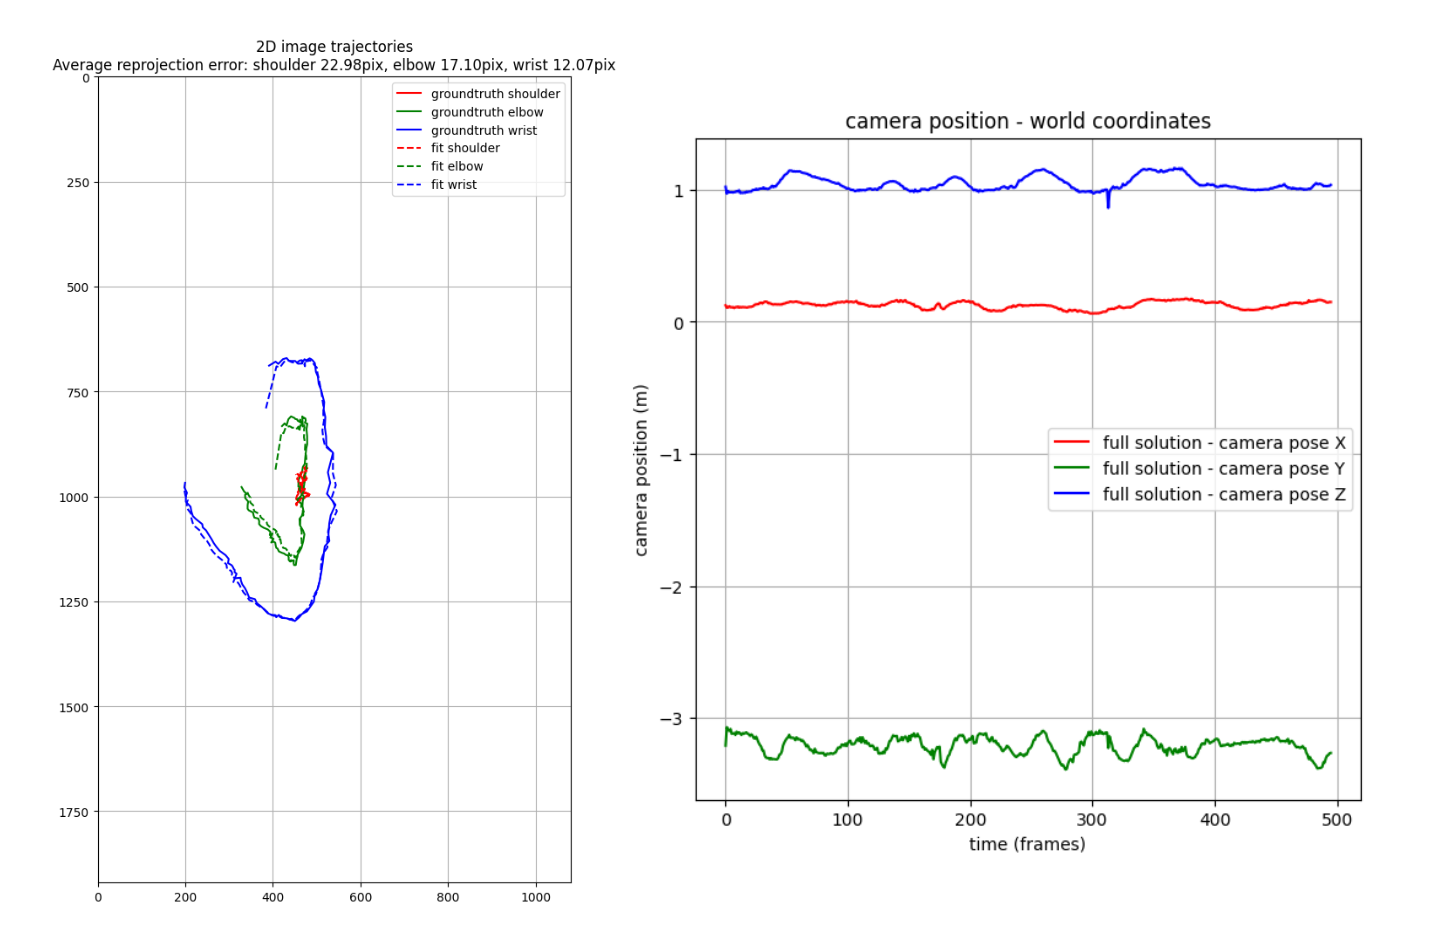
\includegraphics[width=8cm]{figures/camera_pose_fitting_collage.png}
    \caption{Left: projected arm 3D points onto the sensor after camera pose fitting - on the first 100 frames of the video (motion doing a circle with the arm). Average reprojection error reported here are computed on the 3 arm joints over the whole video.
    Right: Estimated distance from the camera to the shoulder is 3 meters wich is faithful to the real distance.}
    \label{fig:camera_fitting}
\end{figure}

\begin{figure*}
    \centering
    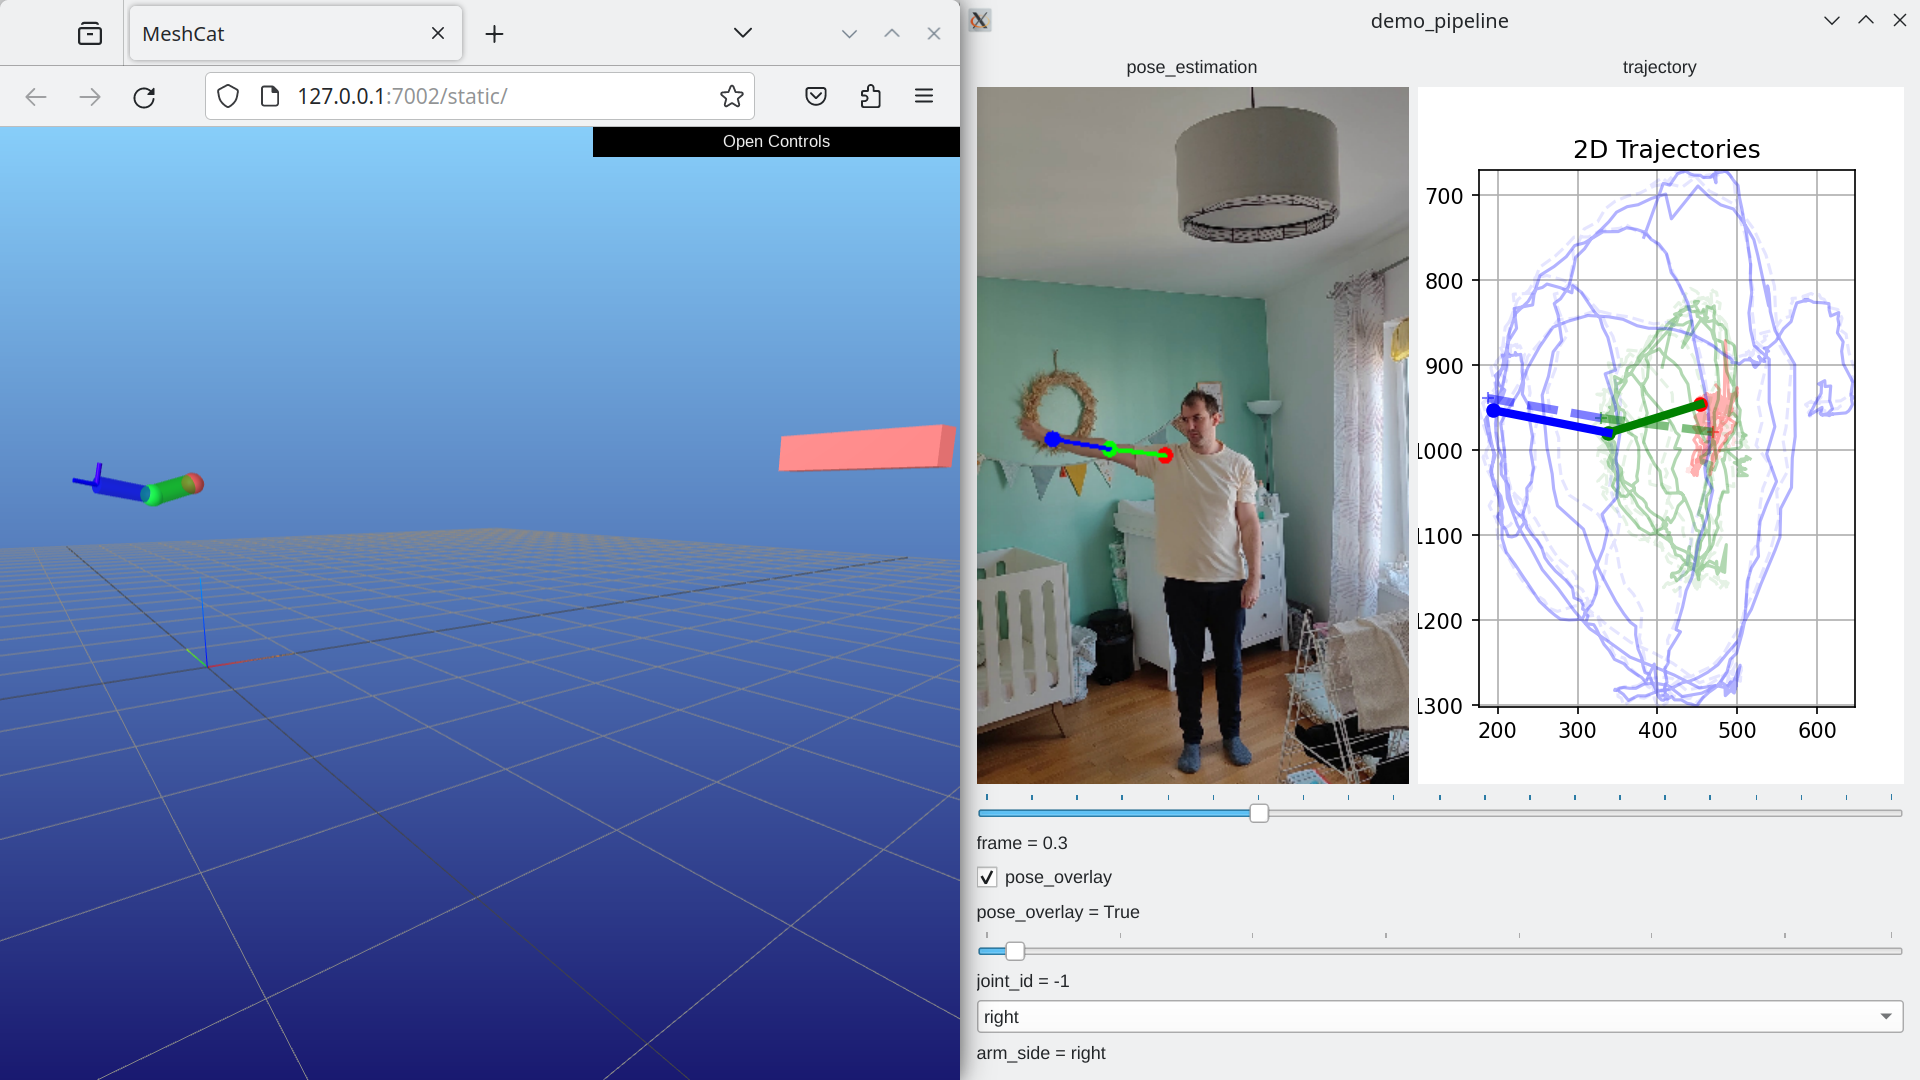
\includegraphics[width=16cm]{figures/arm_demo.png}
    \caption{Demo of the pose estimation pipeline.
    Left: Digital twin of the arm is synchronized witht the GUI. Camera is indicated in pink.
    Right: graphical user interface to select a specific frame
    and visualize the 2D joints position (dashed - right curve) aswell as the 3D reprojection of the arm (plain - right curve).}
    \label{fig:demo}
\end{figure*}

\subsection{Inverse dynamics optimizer}
\label{subsec:inverse_dynamics}

Given the simplifications discussed in~\cref{subsec:arm_model}, we reformulated the optimization problem as follows:

\begin{equation*}
    \begin{aligned}
        & \underset{q,\tau_m}{\text{minimize}} \quad \int_{0}^{T} l(q, \tau_m)\, dt \\
        & \text{subject to} \quad \dot{q} = f(q, \tau_m) \quad \text{(full-arm dynamics)}.
    \end{aligned}
\end{equation*}

\noindent\textbf{Variables.} The model variables consist of the arm's configuration vector \(q\) and the muscle joint torques \(\tau_m\). 
We adopted the central difference scheme to approximate \(\dot{q}\) for its enhanced precision and because it provides velocity information precisely 
at instant \(t\).
\[
    \dot{q}_t = (q_{t + 1} - q_{t - 1}) / 2\Delta t
\]
Acceleration was computed in a similar fashion.

\noindent\textbf{Loss Functions.} Our loss function \(l\) omits \(l_{2D}\) due to the already accurate 3D pose estimates and 
excludes the pose likelihood term since we target only the arm. The remaining terms include:

\begin{itemize}
    \item 
        \(l_{3D}\): Ensures 3D position estimates align with the MediaPipe references.
    \item
        \(l_{\text{torque}}\): A regularization term penalizing high muscle torque values to favor energy-efficient movements.
    \item 
        \(l_{\text{smooth}}\): Motion smoothness.
        This cost term penalizes rapid movements and accelerations.
\end{itemize}

Theses terms are the same than the corresponding ones in~\cref{subsec:reconstruct_original}.

\noindent\textbf{Constraints.} The arm dynamics are governed by the Lagrange dynamics equation:

\[
M(q)\ddot{q} + b(q, \dot{q}) = g(q) + \tau
\].

\noindent\textbf{Implementation.} We discretized the continuous-time problem, 
and use the central difference scheme for derivative approximation. 
Pinocchio facilitated the computation of kinematic and dynamic quantities. 
The optimization was carried out using the Levenberg-Marquardt algorithm implemented in the SciPy library, 
chosen for its ease of integration with our Python-based pipeline. 
Constraint enforcement was achieved by embedding them as penalty terms within the loss function.

\subsection{Inverse Dynamics Results}
\label{subsec:dynamic_results}

Our initial tests of the optimizer were conducted on simulated data, enabling us to assess its performance and fine-tune the loss weights.

\noindent\textbf{Free Fall, Simulated.} We began with a simple free-fall scenario. The arm's initial configuration was horizontal to the ground, with an elbow angle of 
\(\pi/4\) radians. This simulation was performed using the Runge–Kutta 2 method, and the resulting ground truth is depicted 
in~\cref{fig:gt_free_fall}.

\begin{figure}
    \centering
    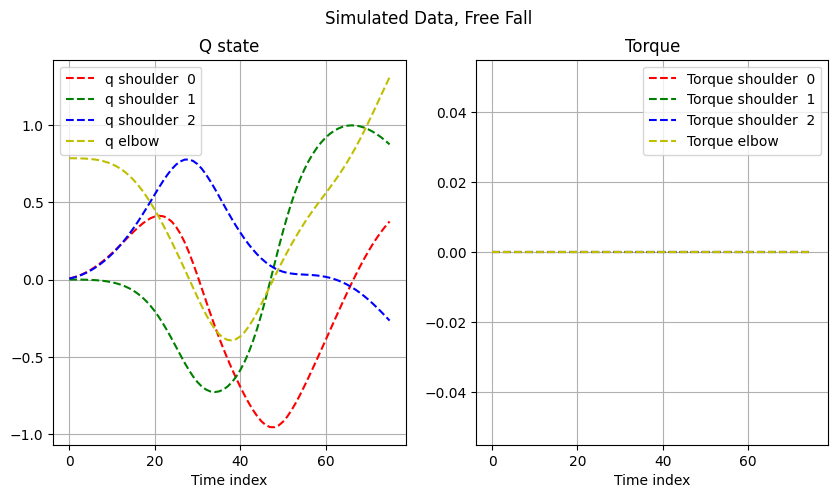
\includegraphics[width=8cm]{figures/free_fall_gt.png}
    \caption{Simulated ground truth data of free fall.}
    \label{fig:gt_free_fall}
\end{figure}

We fed the optimizer with the ground truth 3D poses and initial state vectors \(q_1, \ldots, q_T\) and zero torques. Without torque 
regularization, the optimizer yielded physically implausible torque estimations, despite low pose error, as shown 
in~\cref{fig:free_fall_no_torque}.

\begin{figure}
    \centering
    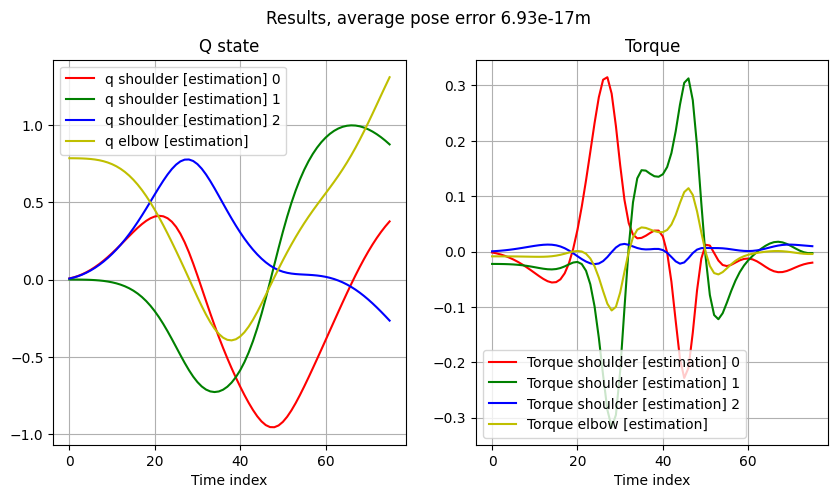
\includegraphics[width=8cm]{figures/free_fall_no_torque.png}
    \caption{Torque estimation without regularization, showing erroneous non-zero torques despite accurate pose estimation.}
    \label{fig:free_fall_no_torque}
\end{figure}

These inaccuracies are attributed to the central difference approximation for velocities and accelerations, and potential undersampling, which 
introduces errors that the optimizer compensates for with non-zero torques.

Incorporating torque regularization significantly improved the results. While the pose error marginally increased, it remained within a 
reasonable range of a few millimeters. Crucially, the torque estimates were much closer to the expected zero value, as illustrated 
in~\cref{fig:free_fall_torque}.

\begin{figure}
    \centering
    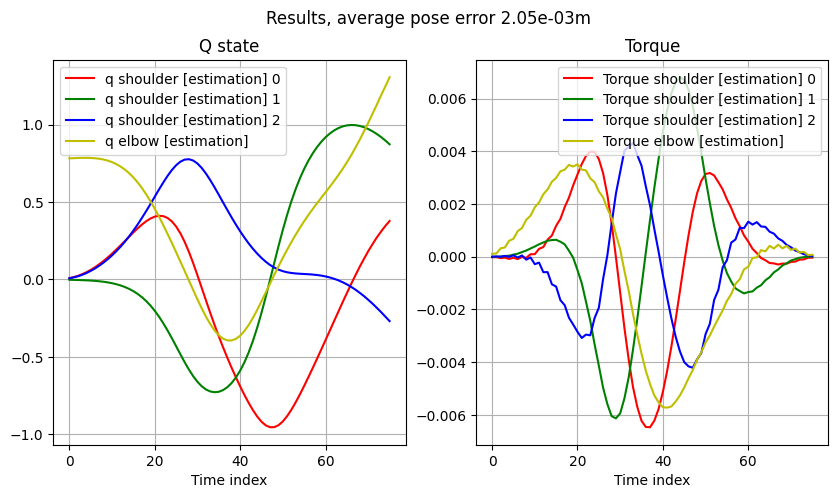
\includegraphics[width=8cm]{figures/free_fall_torque.png}
    \caption{Torque estimation with regularization, showing a pose error still fairly low and torques that align much more closely with the ground truth.}
    \label{fig:free_fall_torque}
\end{figure}

These findings highlight the importance of torque regularization in maintaining physical plausibility, especially when dealing with 
approximations issues.

\noindent\textbf{Free Fall with Friction, Simulated.} We tested the free fall with friction, represented by the equation 
\(\tau_m = -0.1\dot{q}\). This test aimed to evaluate the optimizer's ability to reconstruct non-trivial torque values. Ground truth and results, 
shown in~\cref{fig:free_fall_friction_gt} and~\cref{fig:free_fall_friction}, indicate that while the results are not flawless, 
they demonstrate the optimizer's capability to reconstruct coherent torques.

\begin{figure}
    \centering
    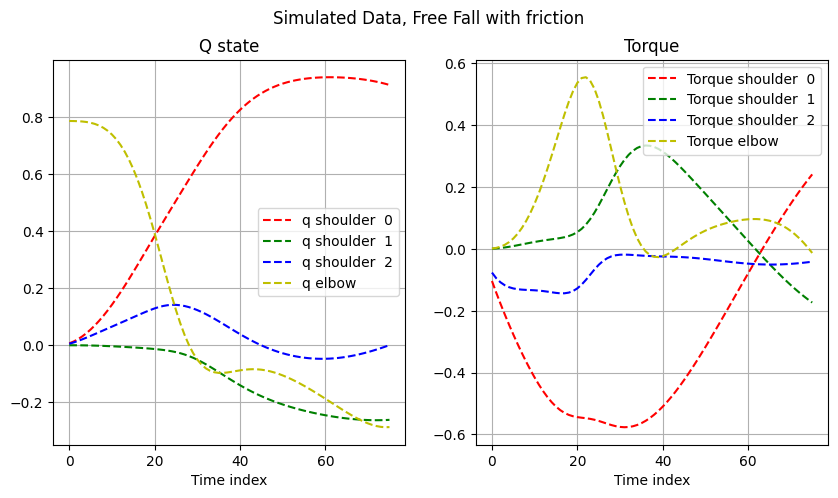
\includegraphics[width=8cm]{figures/free_fall_friction_gt.png}
    \caption{Simulated ground truth data of free fall with friction.}
    \label{fig:free_fall_friction_gt}
\end{figure}

\begin{figure}
    \centering
    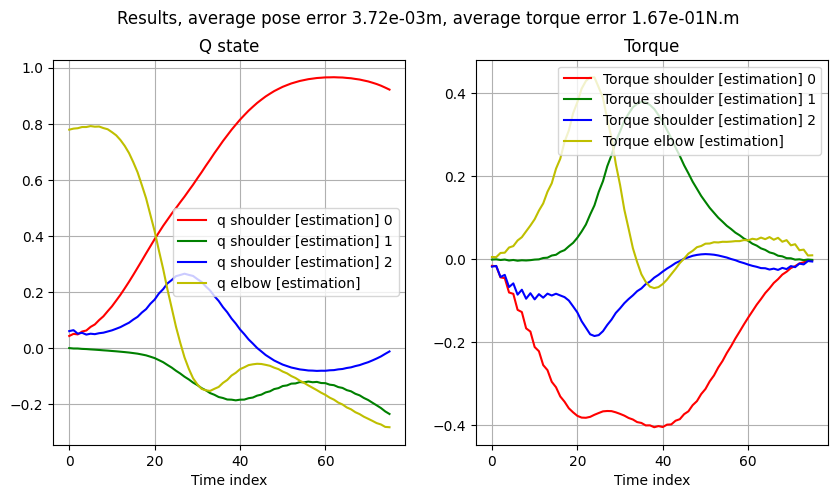
\includegraphics[width=8cm]{figures/free_fall_friction.png}
    \caption{Results of the optimization on the free fall with friction.}
    \label{fig:free_fall_friction}
\end{figure}


\noindent\textbf{Real Data.} When applying our optimizer to real-world data, we encountered several challenges. 
The optimization process in SciPy proved significantly slower on real data, with 2 seconds of video requiring up to 10 minutes of 
computation. Moreover, time constraints and the intricate nature of fine-tuning the loss weights for the optimizer prevented extensive 
testing on real data. Consequently, we could not obtain conclusive results from real-world experiments. We also understand
why the authors of the original paper chose to compile the inverse dynamics optimizer program based on CERES and Pinocchio.
  \section{Discussion on the Paper}
\label{sec:discussion}

Our review and partial reimplementation of the work by~\citet{li2019estimating} have led us to several observations about 
the original study.

\begin{itemize}
    \item \textbf{Method and Code Complexity:} The complexity of the approach, both in terms of the underlying methodology and the associated 
    codebase, poses significant barriers to replication and extension.

    \item \textbf{Simplification of the Vision Pipeline:} The original study uses individual neural network models for each joint in contact recognition
    potentially leading to redundant feature extraction. A more streamlined and modern approach could employ a unified neural network (backbone) to handle 
    these tasks more efficiently. The same remark can be made on the object endpoint detection.

    \item \textbf{Challenging Loss Coefficient Tuning:} Fine-tuning the loss coefficients in the optimization problem presents a significant 
    challenge. The balance between data fidelity and regularization, requires careful calibration, which may 
    limit the method's generalizability to diverse datasets. As there are no clear guidelines on how to tune these coefficients, one can
    assume that the authors fine tuned them to get correct accuracy on the Parkour dataset used for the quantitative evaluation.

    \item \textbf{Confidence in Force and Torque Estimations:} Assessing the accuracy of reconstructed forces and torques is problematic due 
    to the limited benchmarks available for validation. The authors deserve credits for providing quantitative results (based on the Parkour dataset).
    Getting ground truth data for these quantities is very challenging. Realistic simulations do not seem possible.

    \item \textbf{Consistency in Object Weight and Body Dimension Priors:} In their method, weights and weight matrices are predefined. 
    But the movement heavily depends on the weight and dimensions of the manipulated object and the human body, which can vary significantly 
    across different videos. 

    \item \textbf{Relevance of Full Body Dynamics:} Given the necessary approximations in velocity and acceleration, and the inability to 
    strictly enforce full-body dynamics, the added value of attempting to reconstruct these dynamics as opposed to focusing 
    solely on kinematics can be questionned. A comparative analysis with kinematics-focused methods could be insightful.

    \item \textbf{Lack of Data Adimensionality in Optimization:} The absence of adimensionalization or standardization in data processing could 
    affect the model's ability to generalize. This issue becomes particularly evident in scenarios where similar movements are performed at 
    different speeds, potentially leading to varied results.
    One would naturally divide the 2D reprojection errors by the image diagonal size (in pixels), the 3D reprojection errors by the length of the arm,
    the dynamics constraint (torque error) by the static torque of the arm at rest etc... 
    The constants used to weight the cost terms would naturally become more consistent and easier to tune.

    \item \textbf{Torque Regularization:} As discussed in~\cref{subsec:dynamic_results}, the use 
    of \(l_{\text{torque}} = \|\tau_m\|^2\) as a regularization term can lead to suboptimal 
    behavior, particularly in situations where the motion requires significant torques. 
    The simplest correction would be to penalize deviations from the torque obtained in a static configuration deduced from the current state \(l_{\text{torque}} = \|\tau_m - \tau_m^{\textrm{STATIC}} \|^2\).
    Another more appropriate regularization might be on the derivative of the torque, \(\dot{\tau}_m\), which 
    would allow the model to accommodate necessary high torques while still smoothing the energy used in the movement.

\end{itemize}
  \section{Conclusion}
\label{sec:conclusion}

In conclusion, our review and reimplementation of~\citet{li2019estimating}'s paper provided valuable insights into the complexity 
and challenges of estimating 3D motion and forces in human-object interactions from RGB videos. 
The original work stands as a significant novel contribution to this field. While our reimplementation is restricted to a simpler use case,
we still faced a few difficulties, particularly in applying the method to real-world data.
It still allowed us to highlight some limitations of the original method and to propose some improvements.



  \newpage

  %% APPENDIX
  \appendix
  \section{Appendix}
\subsection{Camera calibration}
\label{app:cam_calib}
Since we're working in a controlled environment (not in the wild, unlike the original paper), we calibrate a single camera once and for all,
\begin{itemize}
    \item using a 7x10 printed checkerboard shot in various orientations
    \item  using the OpenCV implementation of the Zhang's method~\cite{Zhang00calib}.
\end{itemize}

Below, we detail the focal length estimation from camera specifications
and make sure it matches with the calibration estimation.
Xiaomi Mi11 Ultra main camera ($2.8\mu m$ pixel pitch) specifications in photo mode:
\begin{itemize}
    \item 24mm focal length - full frame (24x36mm) equivalent
    \item Sensor size 4000x3000 = 12Mpix
\end{itemize}
We end up with a focal length for the photo mode of $f_{\text{pix}}^{\text{photo}}  = 24mm * 4000px / 36mm = 2666px$.

But since we're using a FullHD video mode with a crop factor of around 15\% on each side,
it is needed to rescale the focal length acordingly $f_{\text{pix}}^{\text{video}} = 2666px * 1.3 * \frac{1920px}{4000px} \approx 1664px$.
Calibration method provides a estimated focal length of $1690px$ which is close enough to the specifications.
We assume the camera to be a pinhole and neglect radial distortion.

\subsection{Inverse kinematics}
\label{app:inverse_kinematics}
The goal of Inverse Kinematics applied to our arm problem is to find the $q$ states so that the elbow ($E$) and wrist ($W$)
reach 3D target positions $P_{E}$ and $P_{W}$.
This iterative process is performed by following these steps:
\begin{itemize}
    \item computing the 3D positions of the elbow $\hat{P_{E}}(q)$ and wrist $\hat{P_{W}}(q)$ from the current joint states $q$ using forward kinematics
    \item computing the Jacobians $J_{E}$ and $J_{W}$ of the arm model at the current joint states $q$.
    \item Compute the 3D error vectors 
        \subitem $\Delta_{E} =P_{E} - \hat{P_{E}}(q)$ 
        \subitem $\Delta_{W} =P_{W} - \hat{P_{W}}(q)$. 
    \item We want the elbow to reach the target so we are willing to move the arm with a configuration state increment 
    $\delta q_{E}$ which statisfies $\min_{\delta q_{E}} \|J_{E}.\delta q_{E} - \Delta_{E}\|_2^2.$
    \item This is achieved by computing the pseudo-inverse $J_{E}^+$ of the Jacobian and computing $\delta q_{E} = J_{E}^+ \Delta_{E}$
    \item We also need to move the wrist in the right direction without undoing the elbow movement. This is performed by making an increment for the wrist in the orthogonal null space of the elbow's Jacobian.
    \subitem . Find $\delta q_{W}$ , $\min_{\delta q_{W}\in Ker(J_{E})} \|J_{W} (\delta q_{E} + \delta q_{W}) - \Delta_{W}\|_2^2$
    \subitem . Forcing a vector to be in $Ker(J_{E})$ is achieved using the projection $P_{E}=I-J_{E}^{+}J_{E}$
    \textit{(eg. $\forall \delta q$, $P_{E}.\delta q$ will not change the elbow position)}
    \subitem . $\delta q_{W} = \delta q_{E} + {(J_{W}P_{E})}^{+} (\Delta_{W} - J_{W} \delta q_{E})$
    \item Finally update the joint states $q$ with the increment $\delta q_{W} \Delta T$ where $\Delta T$ defines the convergence speed.
\end{itemize}

Remark: \textit{Jacobian matrix provides the 3D linear velocity 
(and axis-angle angular velocity) at a given joint location when we apply a variation $\delta q_i$ on a specific component $q_i$ of the configuration state $q$.
Note that although the Jacobian provided in Pinocchio provides linear and angular velocities derivatives, we only use the 3D linear velocity part.}

\subsection{Code description}
\label{app:code}
The code is available at:

~\href{https://github.com/balthazarneveu/monocular_pose_and_forces_estimation}{github.com/balthazarneveu/monocular\_pose\_and\_forces\_estimation}

The code is written in Python and relies on a several external libraries:
\begin{itemize}
    \item Pinocchio for kinematics and dynamics computations aswell as the arm model.
    \item Meshcat for 3D visualization.
    \item OpenCV for the camera calibration and the image processing.
    \item MoviePy wraps video processing.
    \item ~\href{https://developers.google.com/mediapipe}{Google Mediapipe} for 2D and  3D pose estimation.
    \item Scipy for the Levenberg-Marquardt optimization.
    \item ~\href{https://github.com/emmcb/batch-processing}{batch-processing} to process multiple video files in a systematic way.
    \item ~\href{https://github.com/balthazarneveu/interactive_pipe}{interactive-pipe} to display a GUI with graphs and images and interact with sliders and keyboard.
    This library works with Matplotlib as the default graphical backend but PyQT/PySide is highly recommended for the demo.
\end{itemize}

To process a new set of videos, located in the \texttt{data} folder, run the following command:
\begin{verbatim}
    python scripts/batch_video_processing.py
    -i "data/*.mp4"
    -o "out"
    -A demo
\end{verbatim}
\textit{When the GUI pops up, press F1 to get the help menu to learn about the shortcuts. Press F11 to display in full screen.
Do not forget to click the hyperlink in the terminal to open the MeshCat viewer in your browser.}


If you're using a different camera, you'll need to calibrate your camera intrinsics first.
Capture a calibration video sequence using a 10x7 checkerboard (print it and stick it on a cardboard or display it on your screen).

\begin{verbatim}
    python scripts/batch_video_processing.py
    -i "data/camera_calibration_<cam_id>.mp4"
    -o "calibration"
    -A camera_calibration
\end{verbatim}

Then you'll be able to process your pose videos using the new camera intrinsics, by simply specifiying
the calibration file path:
\begin{verbatim}
    -calib "calibration/camera_calibration_<cam_id>.yaml"
\end{verbatim}

The core of the code for inverse kinematics and inverse dynamics is located in:
~\href{https://github.com/balthazarneveu/monocular_pose_and_forces_estimation/tree/main/src/projectyl/dynamics}{src/projectyl/dynamics}
  
  \newpage
  %% BIBLIOGRAPHY
  \bibliographystyle{ACM-Reference-Format}
  \bibliography{references}

\end{document}
